\documentclass[conference]{IEEEtran}
\IEEEoverridecommandlockouts
% The preceding line is only needed to identify funding in the first footnote. If that is unneeded, please comment it out.
\usepackage{cite}
\usepackage{amsmath,amssymb,amsfonts}
\usepackage{algorithmic}
\usepackage{graphicx}
\graphicspath{ {./assets/} }
\usepackage{textcomp}
\usepackage{xcolor}
\def\BibTeX{{\rm B\kern-.05em{\sc i\kern-.025em b}\kern-.08em
    T\kern-.1667em\lower.7ex\hbox{E}\kern-.125emX}}
\begin{document}

\title{About Privacy in Internet of Things\\
}

\author{\IEEEauthorblockN{1\textsuperscript{st} Nelson Vieira}
\IEEEauthorblockA{\textit{Faculdade de Ciências Exatas e da Engenharia} \\
\textit{Universidade da Madeira}\\
Funchal, Portugal \\
2080511@student.uma.pt}
}

\maketitle

\begin{abstract}
Internet of things devices are everywhere, since the birth of the idea of ubiquous
computing that human every day life is envisioned containg millions of devices
that control every aspect of our lives. Today we have smart cars, smart houses,
smart cities, wearables among other things that use various types of devices
and various types of networks to communicate, these devices are designed with
usability in mind as a way for us to live a more confortable life. 
One thing that is not though about much is how these devices treat our 
privacy rights. Our information is used, traded and sold without the user
having much say in the matter besides refusing to use these devices or 
not having access to certain features. I propose a system that gives 
the user the crucial information about the devices that are nearby and how
to protect the data that the user doesn't want to share with the systems, this
system is capable of detecting what type of devices are nearby, what kind
of data is collected by these devices and what can be done to protect
unwanted data from being collected.
\end{abstract}

\begin{IEEEkeywords}
privacidade, iot, computação ubíqua, sniffer
\end{IEEEkeywords}

\section{Introdução}
Iot as a term began being used in the 90's, a connection can be drawn
with Mark Weber's article on ubiquous computing and the rise
of devices of various sizes, but mostly the size of a small phone, that
make the idea of Weber a reality. These devices are used in various applications
starting at home with thermostats, fridges, microwaves, getting embeded in cars
in the education system, in our clothes, our phones, watches and even into
space.

Privacy and security might at first appear almost the same thing, but 
privacy is about the user's data and security is about protecting that data.

\section{Trabalhos Relacionados}

\subsection{Privacy Assistants}

There exists a number of privacy assistants in the market. Privacy assistants
have the objective of giving the user flexibility in choosing the
prefered privacy options in available applications, most are used in
smartphones, very few are made for devices in the internet of things. The
university of Carniege Mellon developed one privacy assistant focused on
internet of things called "IoT Assistant" \cite{ColnagoInforming}. This assistant was
created because the designers felt that this part of the market was being
ignored and decided to create it. The creation of this system started with
a user test case to determine the public's knowledge on this matter, it was
tested with a group of 17 people choosed randomly.

\section{Metadologia}

The proposed methology is composed of two phases, the first phase consists of
making a study on the region's general concern with their privacy when
using iot devices, their knowledge of privacy rights, what they do to
protect their privacy rigths. One one side the objective of this study
consist in demistefying the privacy paradox in the region and gather
information about their idea to solve this problem with respect
to iot devices.
The second phase consists in doing an application that can detect iot devices
nearby the user with at least a 10 meters radius. The application should
do the following when detecting a device:
1. it should show some information about the device;
2. it should categorize the device;
3. it should provide the user with privacy options, if the device allows the
user to decline data harvesting.
This application at first sight might appear to be a mere privacy assistant but
it's not, beacause iot assistants merely choose what privacy options
the user first sets and mantains it for every other application that the user
might use. The proposed app doesn't have the objective to conform to the
user's prefered privacy choices, it merely informs the user about nearby iot
devices and can provide the user with privacy options. But the main objective
is creating awareness in individuals about the various devices that are around
and make the user questions their choices.

\subsection{User Awareness}\label{AA}
There has been some work done to determine the users awareness of
their actions online in regard to privacy. An interactive theatre expericence \cite{ColnagoInforming}
was proposed in order to expose privacy malpractices in companies,
specially in the capitalistic world where profit is prioritize
above all else, in this experiment the public is able to interact with
the actors and influence the story of the play, there are various endings depending
on the public's choices throughout the play, some endings the company would
bury the corruption that was going on, in another ending a team of hackers
is able to expose the company's practices to the world. After the play
the team responsible for the experiment would talk with public members about
what they experienced and discussed what was it about and the memebers
pratices with their data on their daily lifes. After some months
the team would talk again with the members that were present in the play and
talk about any changes they have done in the meantime, most said they did 
not change thei behaviour, one member said that it took more care of The
information that made available online because it had a bad expericence before
where some private data was exposed that should have not been exposed. All in 
all the experiment did not prove to be a success in changing people's behaviour.

\subsection{Units}
\begin{itemize}
\item Use either SI (MKS) or CGS as primary units. (SI units are encouraged.) English units may be used as secondary units (in parentheses). An exception would be the use of English units as identifiers in trade, such as ``3.5-inch disk drive''.
\item Avoid combining SI and CGS units, such as current in amperes and magnetic field in oersteds. This often leads to confusion because equations do not balance dimensionally. If you must use mixed units, clearly state the units for each quantity that you use in an equation.
\item Do not mix complete spellings and abbreviations of units: ``Wb/m\textsuperscript{2}'' or ``webers per square meter'', not ``webers/m\textsuperscript{2}''. Spell out units when they appear in text: ``. . . a few henries'', not ``. . . a few H''.
\item Use a zero before decimal points: ``0.25'', not ``.25''. Use ``cm\textsuperscript{3}'', not ``cc''.)
\end{itemize}

\subsection{Equations}
Number equations consecutively. To make your 
equations more compact, you may use the solidus (~/~), the exp function, or 
appropriate exponents. Italicize Roman symbols for quantities and variables, 
but not Greek symbols. Use a long dash rather than a hyphen for a minus 
sign. Punctuate equations with commas or periods when they are part of a 
sentence, as in:
\begin{equation}
a+b=\gamma\label{eq}
\end{equation}

Be sure that the 
symbols in your equation have been defined before or immediately following 
the equation. Use ``\eqref{eq}'', not ``Eq.~\eqref{eq}'' or ``equation \eqref{eq}'', except at 
the beginning of a sentence: ``Equation \eqref{eq} is . . .''

\subsection{\LaTeX-Specific Advice}

Please use ``soft'' (e.g., \verb|\eqref{Eq}|) cross references instead
of ``hard'' references (e.g., \verb|(1)|). That will make it possible
to combine sections, add equations, or change the order of figures or
citations without having to go through the file line by line.

Please don't use the \verb|{eqnarray}| equation environment. Use
\verb|{align}| or \verb|{IEEEeqnarray}| instead. The \verb|{eqnarray}|
environment leaves unsightly spaces around relation symbols.

Please note that the \verb|{subequations}| environment in {\LaTeX}
will increment the main equation counter even when there are no
equation numbers displayed. If you forget that, you might write an
article in which the equation numbers skip from (17) to (20), causing
the copy editors to wonder if you've discovered a new method of
counting.

{\BibTeX} does not work by magic. It doesn't get the bibliographic
data from thin air but from .bib files. If you use {\BibTeX} to produce a
bibliography you must send the .bib files. 

{\LaTeX} can't read your mind. If you assign the same label to a
subsubsection and a table, you might find that Table I has been cross
referenced as Table IV-B3. 

{\LaTeX} does not have precognitive abilities. If you put a
\verb|\label| command before the command that updates the counter it's
supposed to be using, the label will pick up the last counter to be
cross referenced instead. In particular, a \verb|\label| command
should not go before the caption of a figure or a table.

Do not use \verb|\nonumber| inside the \verb|{array}| environment. It
will not stop equation numbers inside \verb|{array}| (there won't be
any anyway) and it might stop a wanted equation number in the
surrounding equation.

\subsection{Some Common Mistakes}\label{SCM}
\begin{itemize}
\item The word ``data'' is plural, not singular.
\item The subscript for the permeability of vacuum $\mu_{0}$, and other common scientific constants, is zero with subscript formatting, not a lowercase letter ``o''.
\item In American English, commas, semicolons, periods, question and exclamation marks are located within quotation marks only when a complete thought or name is cited, such as a title or full quotation. When quotation marks are used, instead of a bold or italic typeface, to highlight a word or phrase, punctuation should appear outside of the quotation marks. A parenthetical phrase or statement at the end of a sentence is punctuated outside of the closing parenthesis (like this). (A parenthetical sentence is punctuated within the parentheses.)
\item A graph within a graph is an ``inset'', not an ``insert''. The word alternatively is preferred to the word ``alternately'' (unless you really mean something that alternates).
\item Do not use the word ``essentially'' to mean ``approximately'' or ``effectively''.
\item In your paper title, if the words ``that uses'' can accurately replace the word ``using'', capitalize the ``u''; if not, keep using lower-cased.
\item Be aware of the different meanings of the homophones ``affect'' and ``effect'', ``complement'' and ``compliment'', ``discreet'' and ``discrete'', ``principal'' and ``principle''.
\item Do not confuse ``imply'' and ``infer''.
\item The prefix ``non'' is not a word; it should be joined to the word it modifies, usually without a hyphen.
\item There is no period after the ``et'' in the Latin abbreviation ``et al.''.
\item The abbreviation ``i.e.'' means ``that is'', and the abbreviation ``e.g.'' means ``for example''.
\end{itemize}
An excellent style manual for science writers is.

\subsection{Authors and Affiliations}
\textbf{The class file is designed for, but not limited to, six authors.} A 
minimum of one author is required for all conference articles. Author names 
should be listed starting from left to right and then moving down to the 
next line. This is the author sequence that will be used in future citations 
and by indexing services. Names should not be listed in columns nor group by 
affiliation. Please keep your affiliations as succinct as possible (for 
example, do not differentiate among departments of the same organization).

\subsection{Identify the Headings}
Headings, or heads, are organizational devices that guide the reader through 
your paper. There are two types: component heads and text heads.

Component heads identify the different components of your paper and are not 
topically subordinate to each other. Examples include Acknowledgments and 
References and, for these, the correct style to use is ``Heading 5''. Use 
``figure caption'' for your Figure captions, and ``table head'' for your 
table title. Run-in heads, such as ``Abstract'', will require you to apply a 
style (in this case, italic) in addition to the style provided by the drop 
down menu to differentiate the head from the text.

Text heads organize the topics on a relational, hierarchical basis. For 
example, the paper title is the primary text head because all subsequent 
material relates and elaborates on this one topic. If there are two or more 
sub-topics, the next level head (uppercase Roman numerals) should be used 
and, conversely, if there are not at least two sub-topics, then no subheads 
should be introduced.

\subsection{Figures and Tables}
\paragraph{Positioning Figures and Tables} Place figures and tables at the top and 
bottom of columns. Avoid placing them in the middle of columns. Large 
figures and tables may span across both columns. Figure captions should be 
below the figures; table heads should appear above the tables. Insert 
figures and tables after they are cited in the text. Use the abbreviation 
``Fig.~\ref{fig}'', even at the beginning of a sentence.

\begin{table}[htbp]
\caption{Table Type Styles}
\begin{center}
\begin{tabular}{|c|c|c|c|}
\hline
\textbf{Table}&\multicolumn{3}{|c|}{\textbf{Table Column Head}} \\
\cline{2-4} 
\textbf{Head} & \textbf{\textit{Table column subhead}}& \textbf{\textit{Subhead}}& \textbf{\textit{Subhead}} \\
\hline
copy& More table copy$^{\mathrm{a}}$& &  \\
\hline
\multicolumn{4}{l}{$^{\mathrm{a}}$Sample of a Table footnote.}
\end{tabular}
\label{tab1}
\end{center}
\end{table}

\begin{figure}[htbp]
\centerline{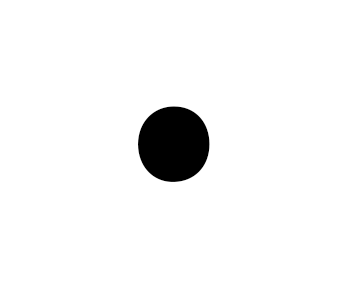
\includegraphics{assets/fig1.png}}
\caption{Example of a figure caption.}
\label{fig}
\end{figure}

Figure Labels: Use 8 point Times New Roman for Figure labels. Use words 
rather than symbols or abbreviations when writing Figure axis labels to 
avoid confusing the reader. As an example, write the quantity 
``Magnetization'', or ``Magnetization, M'', not just ``M''. If including 
units in the label, present them within parentheses. Do not label axes only 
with units. In the example, write ``Magnetization (A/m)'' or ``Magnetization 
\{A[m(1)]\}'', not just ``A/m''. Do not label axes with a ratio of 
quantities and units. For example, write ``Temperature (K)'', not 
``Temperature/K''.

\section*{Agradecimentos}

The preferred spelling of the word ``acknowledgment'' in America is without 
an ``e'' after the ``g''. Avoid the stilted expression ``one of us (R. B. 
G.) thanks $\ldots$''. Instead, try ``R. B. G. thanks$\ldots$''. Put sponsor 
acknowledgments in the unnumbered footnote on the first page.

\section*{References}

Please number citations consecutively within brackets. The 
sentence punctuation follows the bracket. Refer simply to the reference 
number, as in ---do not use ``Ref. '' or ``reference '' except at 
the beginning of a sentence: ``Reference was the first $\ldots$''

Number footnotes separately in superscripts. Place the actual footnote at 
the bottom of the column in which it was cited. Do not put footnotes in the 
abstract or reference list. Use letters for table footnotes.

Unless there are six authors or more give all authors' names; do not use 
``et al.''. Papers that have not been published, even if they have been 
submitted for publication, should be cited as ``unpublished''. Papers 
that have been accepted for publication should be cited as ``in press''. 
Capitalize only the first word in a paper title, except for proper nouns and 
element symbols.

For papers published in translation journals, please give the English 
citation first, followed by the original foreign-language citation. \cite{ColnagoInforming}

\bibliographystyle{IEEEtran}
\bibliography{assets/references}

\end{document}
